A complex system is generally characterized by variability and neurons make no
exception. In this setting, variability refers to changes in some measurable quantities,
such as the spike timing. The main type of variability is the trial-to-trial one, which
can be observed across repetitions of the same experiment.
\begin{figure}[H]
    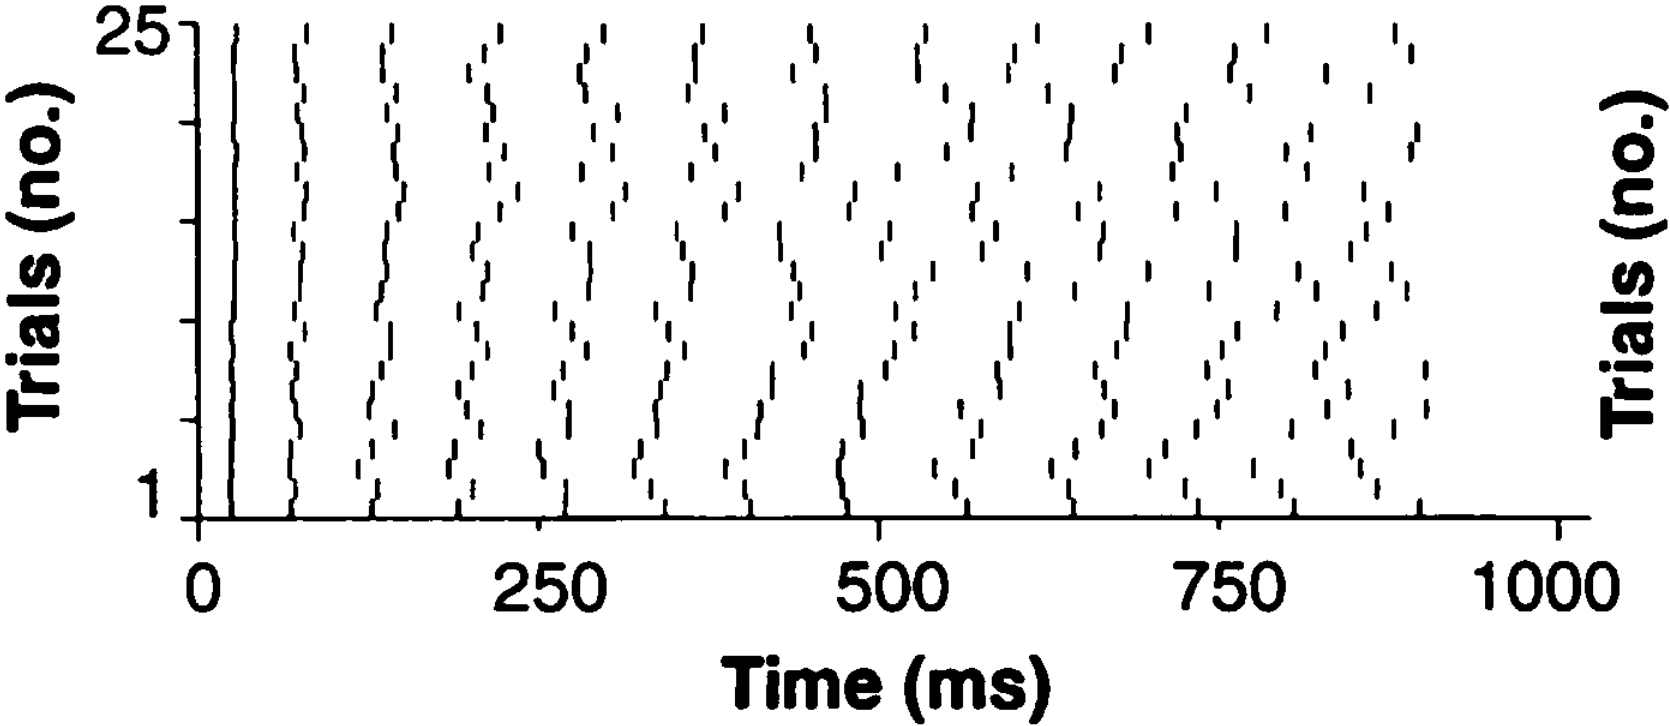
\includegraphics[scale=0.3]{08_1}
    \centering
\end{figure}
The sources of trial-to-trial variability are mainly two:
\begin{enumerate}
    \item \textbf{Deterministic properties of the system}: the initial state of the
          neuronal circuit might not be always the same.
    \item \textbf{Noise}: it is defined as random or unpredictable fluctuations
          and disturbances not belonging to the signal, which can be addictive or distort
          the signal. Noise is a crucial issue in information processing.
\end{enumerate}
Noise can be categorized into several types according to its statistical properties.
A partial solution might consist in filtering out some of the noise; on the other hand,
it might be important to investigate how and where such noise is originated.\\
The main sources of noise in the nervous system are reported in this schema.
\begin{figure}[H]
    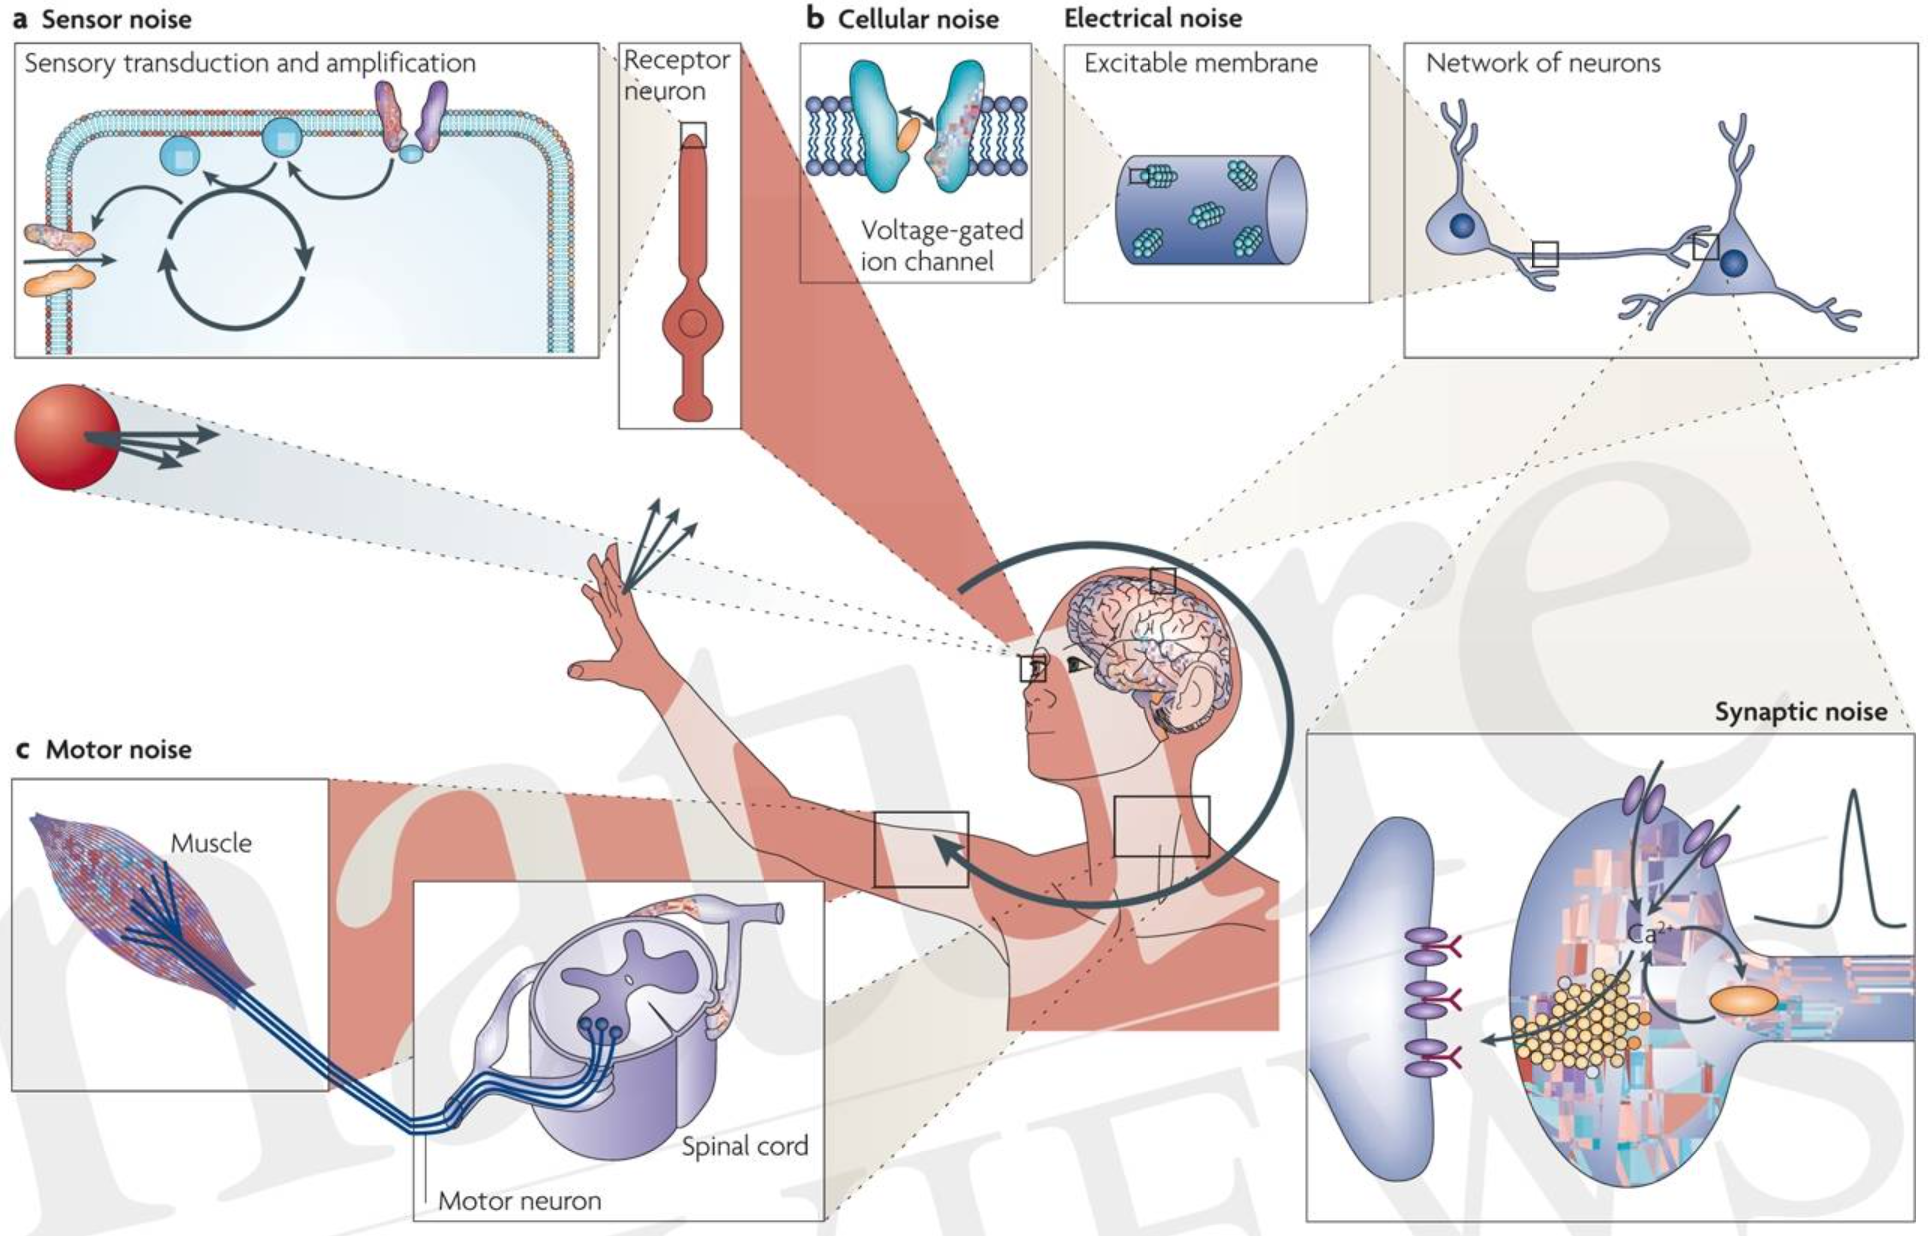
\includegraphics[scale=0.32]{08_2}
    \centering
\end{figure}
\paragraph{Sensory Noise} External sensory stimuli are intrinsically noisy. In particular,
they are converted from several distinct domains, such as the electromagnetic one in the
case of photoreceptors, into chemical or mechanical signals. Then, such signal is amplified
and converted into an electrical one. In addition, it has been observed that stimulating
neurons with a constant stimulus, for instance a DC current, is all but natural, as real world
stimuli are far from being constant and steady; on the contrary, a natural stimulus does not
provide constant features, thus the nervous system is used to deal with noisy inputs and
extract useful information from them.
\paragraph{Cellular Noise} If neurons are driven with identical constant stimuli over repeated
trials, the timing of the elicited action potentials varies across the trials. Such a variability
is in the order of \(ms\), or even lower, but it drastically affects the capability of neurons
to detect coincident signals or their order of arrival.\\
Note that the neuronal activity might look random without actually being random. Even if the
statistical characteristics of neuronal variability resemble the ones typical of a random process,
it does not necessarily mean that the firing pattern observed is generated by such a random process.
Shannon's theory of information states that when the optimal encoding is used to maximize information
transmission, the signal will look random.

\subsection{Sources of Cellular Noise}
\paragraph{Electrical Noise} This kind of noise causes membrane potential fluctuations, either with
or without synaptic inputs. Most of the electrical noise in a cell is channels noise, which is
made of electrical currents produced by the random opening and closing of ion channels.\\
Note that if \(N\) channels are considered, the coefficient of variation \(CV\) is computed
as follow:
\begin{equation*}
    CV=\sqrt{\frac{variance}{mean}}=\sqrt{\frac{1-p(V)}{N\cdot{p(V)}}}
\end{equation*}
Therefore, it can be stated that \(CV\propto{\frac{1}{\sqrt{N}}}\), hence the noisiness of a membrane current
declines proportionally to the square root of the number of channels \(N\).
\begin{figure}[H]
    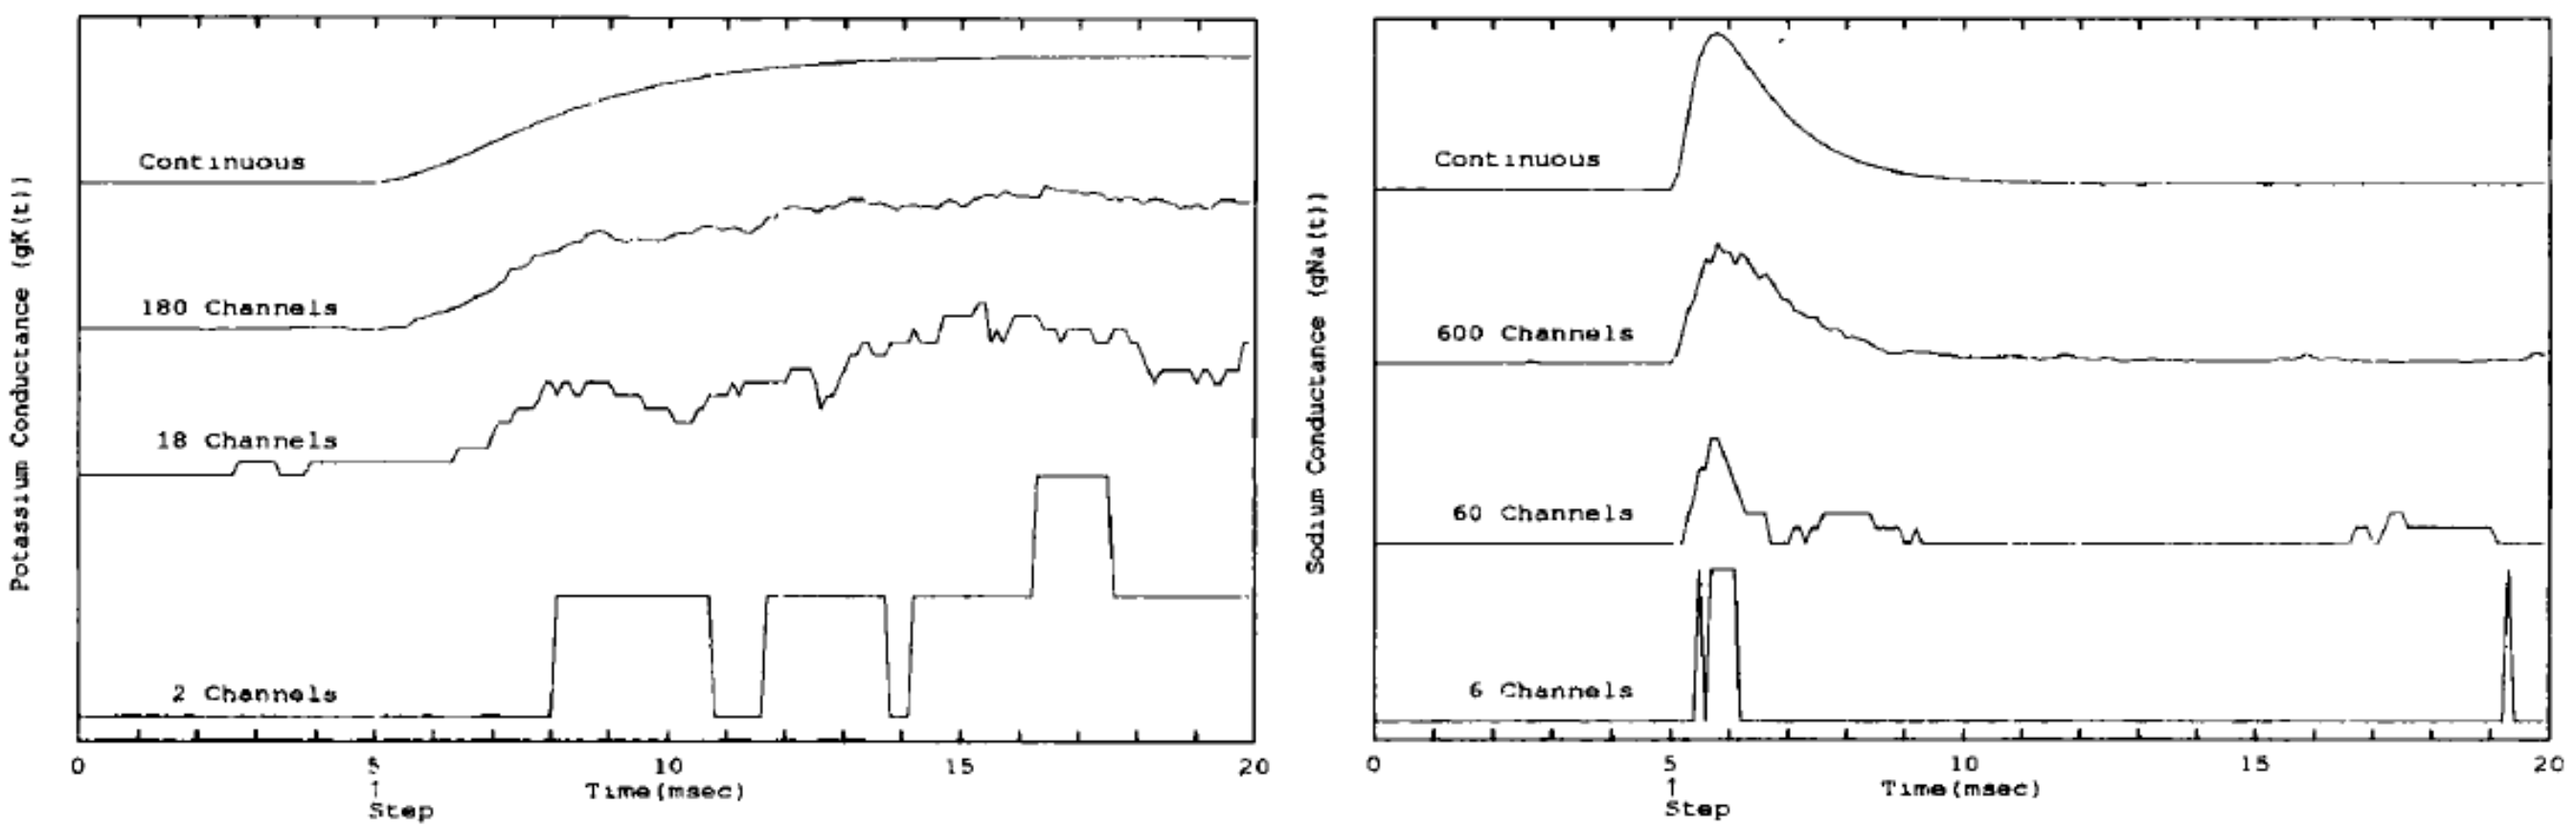
\includegraphics[scale=0.275]{08_3}
    \centering
\end{figure}
As already observed, if \(N\) is small, then the variability of a single channel is very high, but if a large
set of channels is taken into account, the model tends to be compliant with the Hodgkin-Huxley model, which
is deterministic and does not take into account noise.
\paragraph{Johnson Noise} It is related to the temperature and is generated by the thermal agitation of charge
carriers inside an electrical conductor. It is dependent on the material considered.
\paragraph{Shot Noise} This is a type of noise whenever the amount of signal particles (such as electrons or ions
in an electrical circuit or photons hitting a photoreceptor) is small enough to give rise to detectable
statistical fluctuations in a measurement, not enabling a correct and reliable esteem of the incoming
information.
\paragraph{Synaptic Noise} Synapses are always releasing a certain quantity of neurotransmitters
(synaptic bombardment), some of them might evoke some kind of response in the post-synaptic terminal
(spontaneous miniature post-synaptic current or mPSC) even if no
action potential was fired. This kind of noise is diffuclt to address, as multiple sources are involved.
In addition, the relevance of this phenomenon is greater in highly connected neurons, as the integration
effect of neurotransmitters coming from all of the available synapses is no longer negligible.

\subsection{Reliability and Noise}
Despite the brain noise, it has been shown that such noise plays a fundamental role in neural
information processing. It enhances the reliability and regularity of neuronal firing both
in single neurons and populations. Researchers demonstrated that a constant DC stimulation
generated firing patterns with a considerable variability across trials, while if random
noisy fluctuations are superimposed on such a stimulus, then the reliability of spikes
is enormously improved. This can be explained by saying that natural inputs are in fact noisy
and the nervous system is therefore designed to work with them.
\begin{figure}[H]
    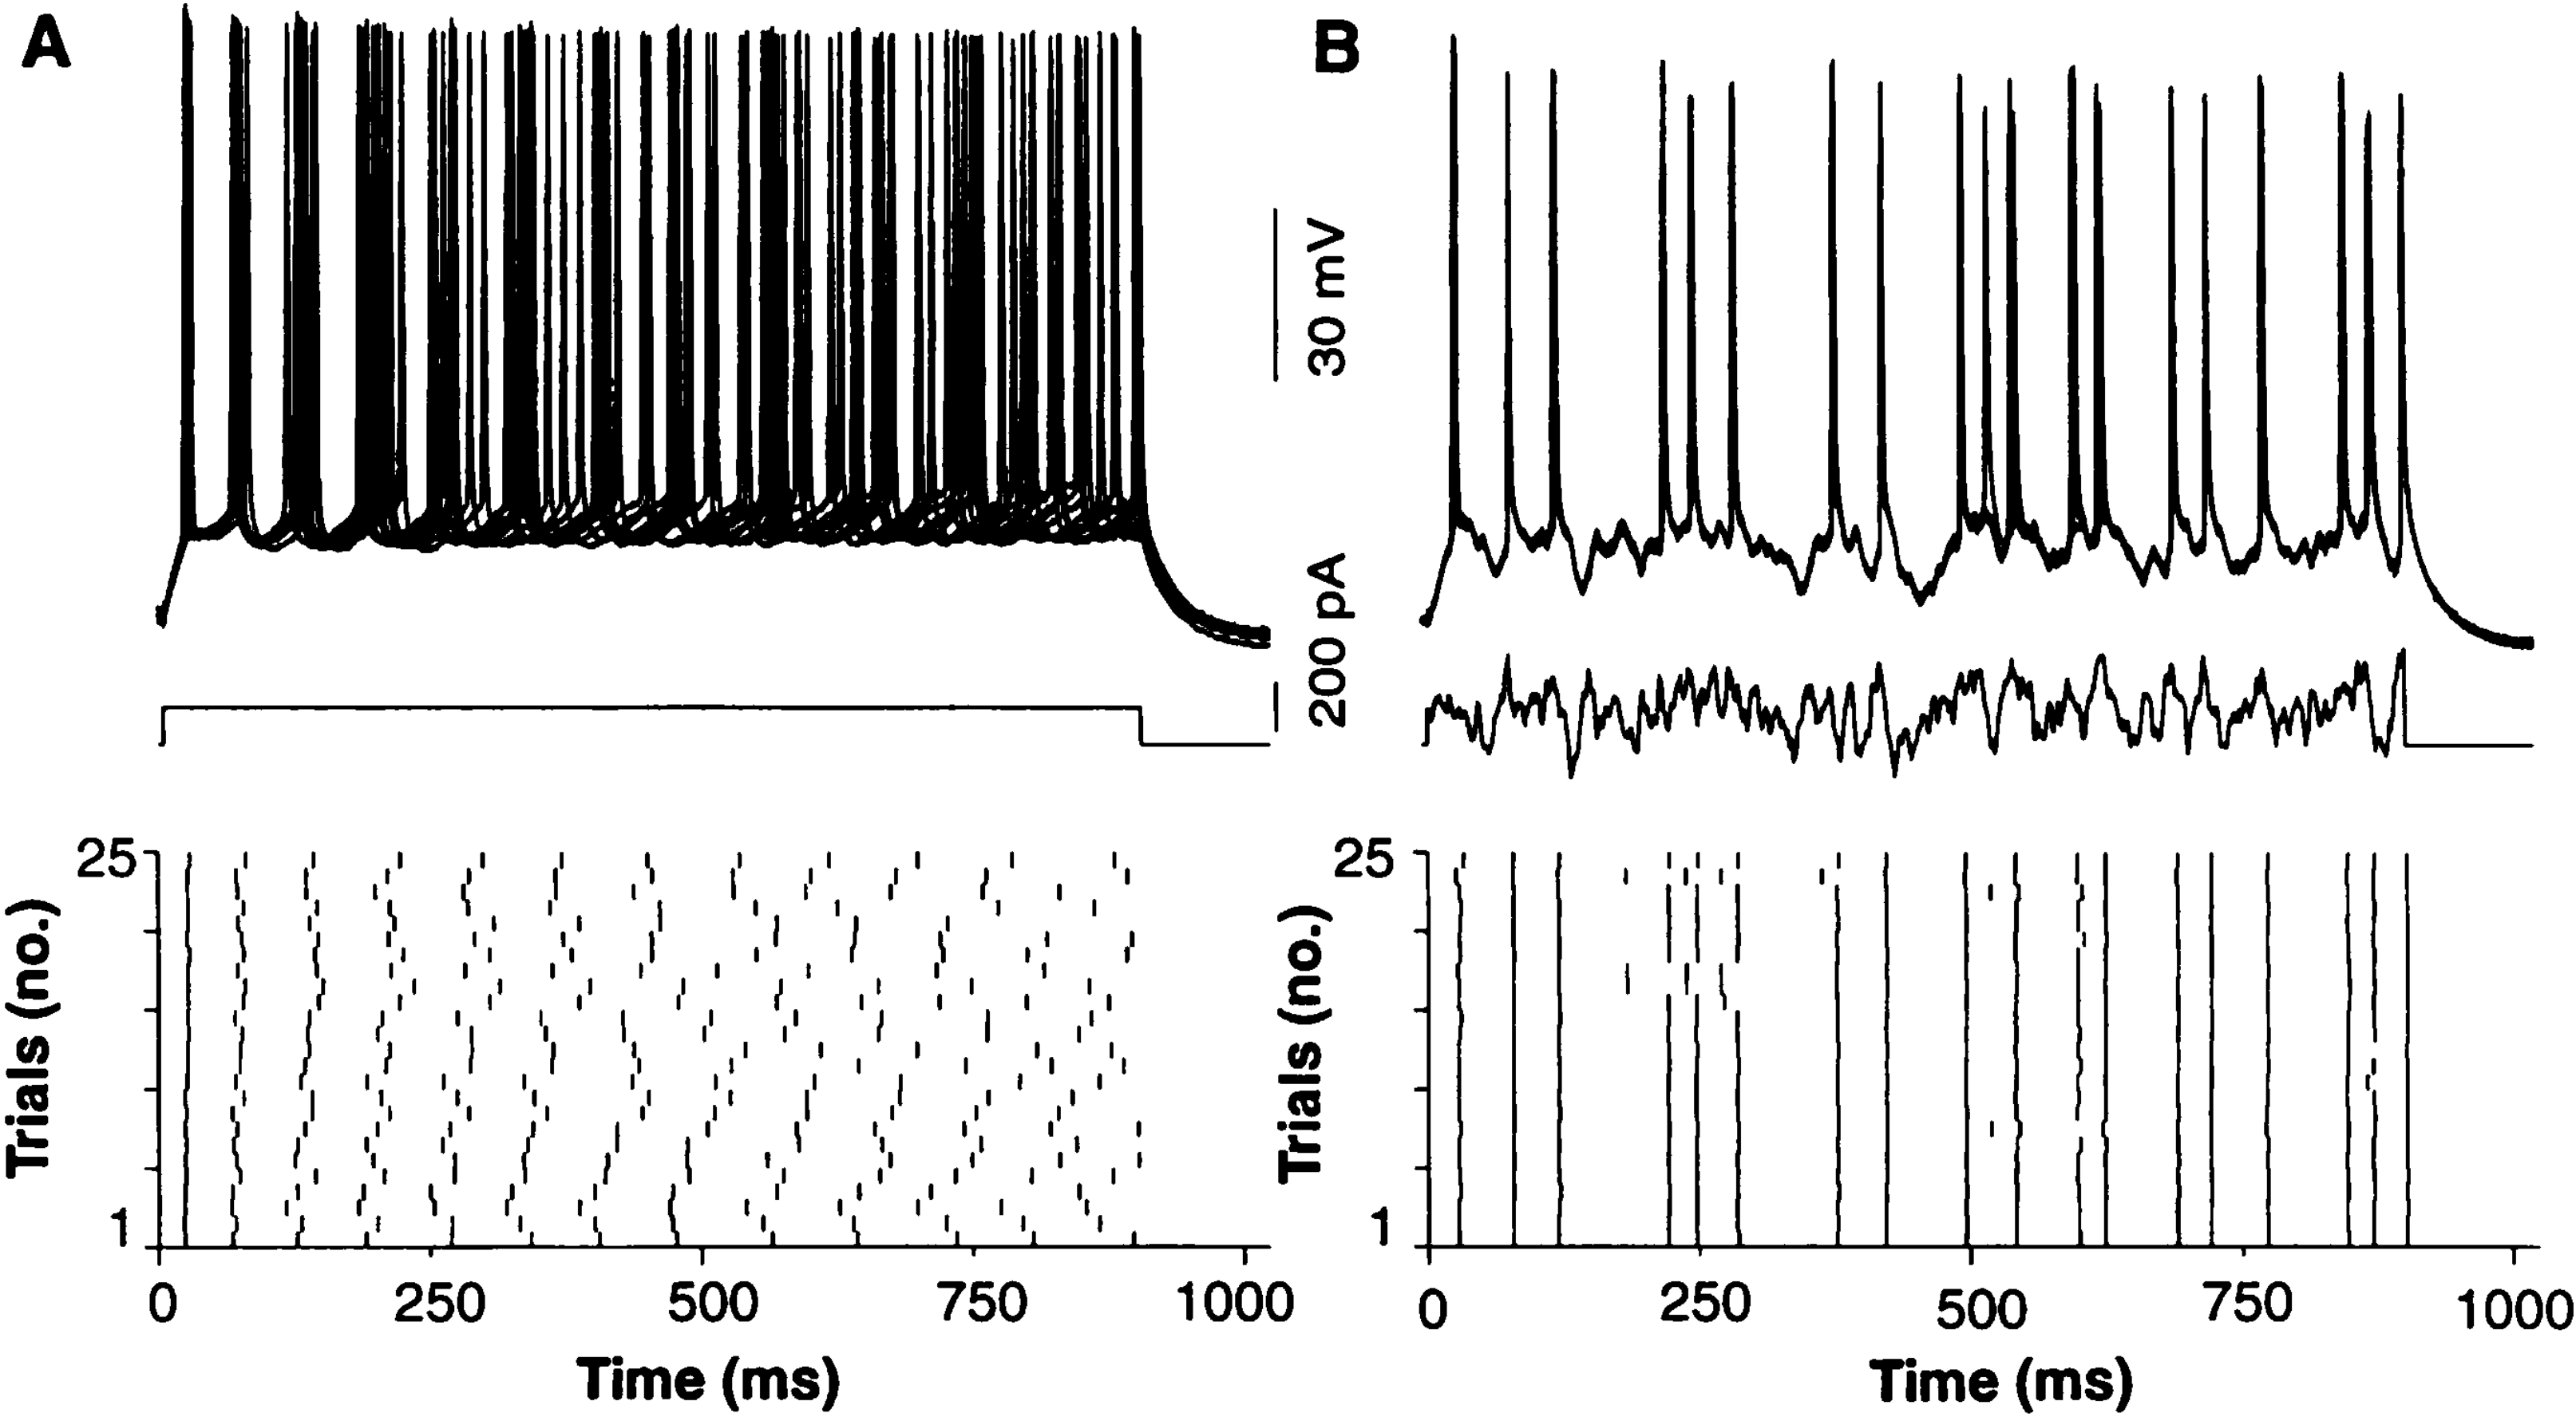
\includegraphics[scale=0.24]{08_4}
    \centering
\end{figure}
Neurons fire in a clock-like fashion, with spikes being separated by fixed time intervals.
Noise facilitates this spiking periodicity.
\begin{itemize}
    \item \textbf{Stochastic Resonance}: if a neuron receives a sub-threshold time-varying input,
          then the addition of noise induces action potentials only during the peaks of such signal,
          when the activation threshold is overcome.
    \item \textbf{Coherence Resonance}: in this case neurons receive exclusively noise with a
          supra-threshold amplitude. The response is thus more synchronized, with \(CV\to{0}\).
\end{itemize}
To sum up, it should be highlighted that noise is crucial when dealing with neurons. Hence,
when building a model (at any scale) it is vital to properly take into account noisy
components. This is particularly true when the investigated topic is the coding capability of
a neuron, as coding cannot neglect the effect of spontaneous fluctuations.